\documentclass[aspectratio=43]{beamer}
\usepackage[utf8]{inputenc}
\usepackage[T1]{fontenc}
\usepackage{xcolor}
\usetheme{anl}

\usepackage[square,sort]{natbib}
\setbeamerfont{footnote}{size=\tiny}
\setbeamerfont{footnote mark}{size=\tiny}
\setbeamerfont{caption}{size=\scriptsize}
\setbeamerfont{cite}{size=\tiny}
% To override the ANL theme.
%\newenvironment{plainblock}[1]{%
%	\setbeamercolor{block body}{bg=white,fg=white}
%	\setbeamertemplate{blocks}[rounded][shadow=false]
%	\begin{block}{#1}}{\end{block}}

\title{High performance implementation of tomography inversion with error correction}
%\subtitle{But they do get pretty big\ldots}
\date[SASSy]{\textbf{S}ummer \textbf{A}rgonne \textbf{S}tudent \textbf{Sy}mposium, 8/28/20}
%%\author[Sajid]{Sajid Ali}
\author[Sajid]{Sajid Ali, Advisors: Zichao Wendy Di \& Matthew Otten}
\coverphoto{graphics/anl-aerial.jpg}

%% Used guidance from: https://tex.stackexchange.com/questions/146529/design-a-custom-beamer-theme-from-scratch

\begin{document}

\begin{frame}
\titlepage
\end{frame}

%\begin{frame}{Outline}
%\tableofcontents
%\end{frame}

\section{Tomography}
\begin{frame}{Basics}
	\begin{block}{}
    \begin{itemize}
    	\item Radon transform : Real $\rightleftarrows$ Sinogram space.
    	\item $Rf(\tau,\theta) = 
    	 \int_{-\infty}^{\infty}\int_{-\infty}^{\infty}
    	 f(x,y)\delta(\tau - x cos(\theta) - y sin(\theta))dxdy $
	\end{itemize}
    \end{block}
	\begin{center}
		\begin{figure}
			\includegraphics[scale=0.335]{figures/ppa_combined.png}
			\caption{Spinning the object to obatin "sinograms", reconstruct each slice independently. Figure taken from \cite{jacobsen_2019}}
		\end{figure}
	\end{center}
	
\end{frame}

\begin{frame}{Center of rotation drifts}
\begin{columns}[onlytextwidth,T]
	\column{\dimexpr\linewidth-45mm}
	\begin{block}{}
	\begin{itemize}
		\item $P_{\theta} = x_{\theta}^{*}(1-cos(\theta) + y_{\theta}^{*}sin(\theta))$ 
		\item $Rf(\tau,\theta,0,0) = Rf(\tau - P_{\theta},\theta,x_{\theta}^{*},y_{\theta}^{*})$
		\item Translation of sinogram by $P_{\theta}$ achieved by convolution with Gaussian.
		\item Recover $P_{\theta}$ to obtain accurate reconstruction as shown in \cite{wendy_2019}
	\end{itemize}					
	\end{block}
	\column{40mm}
	\begin{figure}
		\includegraphics[width=45mm]{figures/drifts.png}
		\caption{Center of rotation drift causes us to measure the shifted sinograms, figure from \cite{wendy_2019}}
	\end{figure}
	\end{columns}
\end{frame}

\section{Algorithm}

\begin{frame}{Optimization formulation}
	\begin{block}{Discretize \& Vectorize}
		\begin{itemize}
			\item $\mathcal{W}$ : object vector
			\item $\mathcal{L}$ : discretized Radon transform
			\item $\mathcal{D}$ : measure sinogram
		\end{itemize}
	\end{block}
	\begin{exampleblock}{Least squares cost function}
		\begin{itemize}
			%\item Assuming no shifts, we need
			%$\underset{\mathcal{W} \geq 0}{\textit{min}}  %\frac{1}{2}||\mathcal{L}\mathcal{W}-\mathcal{D}||$
			\item To recover both shifts and object : 
			$\underset{\mathcal{W} \geq 0, P_{\theta}}{\textit{min}}  \phi(\mathcal{W},P_{\theta}) = \frac{1}{2}||\mathcal{L}\mathcal{W} - g(\mathcal{D},P_{\theta})||$
			\item First order derivatives analytically computable :
			$ \nabla \phi(\mathcal{W},P_{\theta}) = [\mathcal{L}^{T},
			\nabla_{P_{\theta}} \phi(\mathcal{W},P_{\theta})]^{T} (\mathcal{L}\mathcal{W} - g(\mathcal{D},P_{\theta}))$
		\end{itemize}
	\end{exampleblock}
\end{frame}

\begin{frame}{Implementation}
	\begin{block}{}
		\begin{itemize}
			\item Implemented in C/C++ using :
			\begin{itemize}
				\item PETSc (optimization routines, data management and parallel I/O)
				\item Boost (geometry routines) 
				\item FFTW (fourier space convolution)
			\end{itemize}
		\end{itemize}
	\end{block}
	\begin{block}{Joint}
		\begin{itemize}
			\item Combine shifts and sample into one vector and optimize for both together.
		\end{itemize}
	\end{block}
	\begin{exampleblock}{Alternating}
		\begin{itemize}
			\item Alternate between optimizing with respect to sample and with respect to shifts.
		\end{itemize}
	\end{exampleblock}
\end{frame}

\section{Results}
\begin{frame}{Accuracy}
		\begin{center}
		\begin{figure}
			\vspace*{-0.75cm}\hspace*{-1.5cm}\includegraphics[scale=0.225]{figures/func_resd.pdf}
			\caption{Dimensions of unknowns : $800+4096x4096$, size of sinogram : $4096x800$}
		\end{figure}
	\end{center}
\end{frame}
\begin{frame}{Scaling}
	\begin{center}
		\begin{figure}
			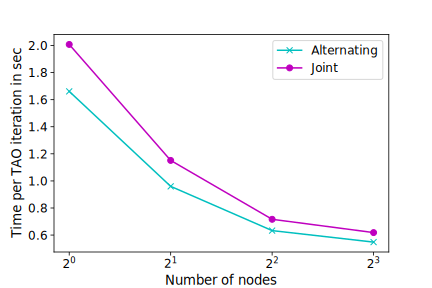
\includegraphics[scale=0.6]{figures/basic_scaling.pdf}
			\caption{Strong scaling plots for alternating and joint reconstruction algorithms performned on bebop (dual socket broadwell), problem size : 2048x2048+400 unknowns.} 
		\end{figure}
	\end{center}
\end{frame}

\section{Future}
\begin{frame}{Summary}
  \begin{block}{Tasks completed}
  \begin{itemize}
  \item Refactor \& fix several bugs.
  \item Profiling : most of solve is spent doing MatMult \& MatMultTranspose
  \item Minor performance enhancements
  \end{itemize}
  \end{block}
  \begin{exampleblock}{Ongoing \& Planned}
  \begin{itemize}
  \item Port application to GPU : premliminary results show reduction in solve time but load balance becomes challenging.
  \item Invert 3D tomography data by replicating the 2D solve on sub-communicators.
  \end{itemize}	
  \end{exampleblock}
	
\end{frame}

{\usebackgroundtemplate{
		\includegraphics[width=\paperwidth,height=0.9\paperheight]{graphics/closing.png}} 
\begin{frame}
\begin{center}
\begin{itemize}
	\item[] {\Large \textcolor{white}{Thank you!}}
\end{itemize}			
\end{center}
%\vspace{0.3cm}
\paragraph{\textbf{\textcolor{white}{Acknowledgements:}}}
\begin{itemize}
	\item \textcolor{white} {Matthew Kehoe}
	\item \textcolor{white} {PETSc-developers and PETSc-Users mailing list for advice, bug fixes and features.}
\end{itemize}
\end{frame}
}
\renewcommand*{\bibfont}{\scriptsize}
\begin{frame}[t, allowframebreaks]
	\frametitle{References}
	\bibliographystyle{dinat-etal}
	\bibliography{pirt}
\end{frame}

\end{document}
